% answers.tex —— 2000 年·春季上海卷 · 参考答案与详细解析片段
% 由 tools/generate_projects.py 依来源总账自 2000/2000_数学真题_春季上海_试题.md + 2000/2000_数学真题_春季上海_解析正文.md + 2000/2000_数学真题_春季上海_答案要点.md 生成，勿手改（改源 MD 后重跑）


\begin{gktip}
以下解析依据已盲核题面独立推导，已由两路独立求解者交叉复算，并与固定扫描件印刷附录逐题比对；不代表官方解析。附录来源身份未核实，不视为官方权威。三幅题图已矢量重绘并局部核对，正式构建尚未完成。
\end{gktip}

\gkpart{一、填空题}

\begin{answer}
\gksolhead{1}{}

\textbf{题目}：

若 $\sin\left(\dfrac{\pi}{2}+\alpha\right)=\dfrac{3}{5}$，则 $\cos 2\alpha=\underline{\qquad}$。

\Needspace{4\baselineskip}
\textbf{解析}

\Needspace{5\baselineskip}
由 $\sin\left(\dfrac\pi2+\alpha\right)=\cos\alpha=\dfrac35$，得

\nopagebreak[4]
\[
\cos2\alpha=2\cos^2\alpha-1=2\cdot\frac9{25}-1=-\frac7{25}.
\]

\gkanswer{答案：$-\dfrac{7}{25}$。}

\end{answer}
\begin{answer}
\gksolhead{2}{}

\textbf{题目}：

若函数 $f(x)=\dfrac{x}{x+2}$，则 $f^{-1}\left(\dfrac{1}{3}\right)=\underline{\qquad}$。

\Needspace{4\baselineskip}
\textbf{解析}

令 $y=\dfrac{x}{x+2}$，则 $yx+2y=x$，从而 $x=\dfrac{2y}{1-y}$（$y\ne1$）。故 $f^{-1}\left(\dfrac13\right)=1$。

\gkanswer{答案：$1$。}

\end{answer}
\begin{answer}
\gksolhead{3}{}

\textbf{题目}：

方程 $\log_4(3x-1)=\log_4(x-1)+\log_4(3+x)$ 的解是 $\underline{\qquad}$。

\Needspace{4\baselineskip}
\textbf{解析}

\Needspace{5\baselineskip}
定义域要求 $3x-1>0$、$x-1>0$、$x+3>0$，合并得 $x>1$。于是

\nopagebreak[4]
\[
3x-1=(x-1)(x+3),
\]

即 $(x-2)(x+1)=0$。结合定义域只取 $x=2$。

\gkanswer{答案：$x=2$。}

\end{answer}
\begin{answer}
\gksolhead{4}{}

\textbf{题目}：

若 $(\sqrt{x}+a)^5$ 的展开式中的第四项是 $10a^2$（$a$ 为大于零的常数），则 $x=\underline{\qquad}$。

\Needspace{4\baselineskip}
\textbf{解析}

\Needspace{5\baselineskip}
按 $\sqrt{x}$ 的降幂展开，第四项为

\nopagebreak[4]
\[
\binom53(\sqrt{x})^2a^3=10xa^3.
\]

由 $10xa^3=10a^2$ 且 $a>0$，得 $x=\dfrac1a$。

\gkanswer{答案：$x=\dfrac{1}{a}$。}

\end{answer}
\begin{answer}
\gksolhead{5}{}

\textbf{题目}：

在三角形 $ABC$ 中，$\sqrt{2}\sin A=\sqrt{3\cos A}$，则 $\angle A=\underline{\qquad}$。

\Needspace{4\baselineskip}
\textbf{解析}

\Needspace{5\baselineskip}
因右边为实数，须有 $\cos A\ge0$；对原等式平方得

\nopagebreak[4]
\[
2\sin^2 A=3\cos A
\quad\Longrightarrow\quad
2\cos^2 A+3\cos A-2=0.
\]

可行根为 $\cos A=\dfrac12$（另一根 $-2$ 不可能），故 $A=60^\circ$。

\gkanswer{答案：$60^\circ$。}

\end{answer}
\begin{answer}
\gksolhead{6}{}

\textbf{题目}：

若直线 $l$ 的倾角为 $\pi-\operatorname{arctg}\dfrac{1}{2}$，且过点 $(1,0)$，则直线 $l$ 的方程为 $\underline{\qquad}$。

\Needspace{4\baselineskip}
\textbf{解析}

\Needspace{5\baselineskip}
直线斜率为 $\tan\left(\pi-\arctan\dfrac12\right)=-\dfrac12$。过 $(1,0)$，故

\nopagebreak[4]
\[
y=-\frac12(x-1),\qquad x+2y-1=0.
\]

\gkanswer{答案：$x+2y-1=0$。}

\end{answer}
\begin{answer}
\gksolhead{7}{}

\textbf{题目}：

若数列 $\{a_n\}$ 的通项为 $a_n=\dfrac{1}{n(n+1)}$（$n\in\mathbb{N}$），则 $\displaystyle\lim_{n\to\infty}(a_1+n^2a_n)=\underline{\qquad}$。

\Needspace{4\baselineskip}
\textbf{解析}

\nopagebreak[4]
\[
a_1+n^2a_n=\frac12+\frac{n}{n+1}\longrightarrow\frac32.
\]

\gkanswer{答案：$\dfrac{3}{2}$。}

\end{answer}
\begin{answer}
\gksolhead{8}{}

\textbf{题目}：

如图，$\angle BAD=90^\circ$ 的等腰直角三角形 $ABD$ 与正三角形 $CBD$ 所在平面互相垂直，$E$ 是 $BC$ 的中点，则 $AE$ 与平面 $BCD$ 所成角的大小为 $\underline{\qquad}$。
\nopagebreak[4]
\begin{center}% Q8 原图几何关系的空间示意；不表示各边实际比例。
% 构形：BD=2，C=(1,sqrt(3),0)，A=(1,0,1)，仅用于满足题设关系。
% right angle: BAD; midpoint: E on BC; perpendicular planes: (ABD) and (BCD).
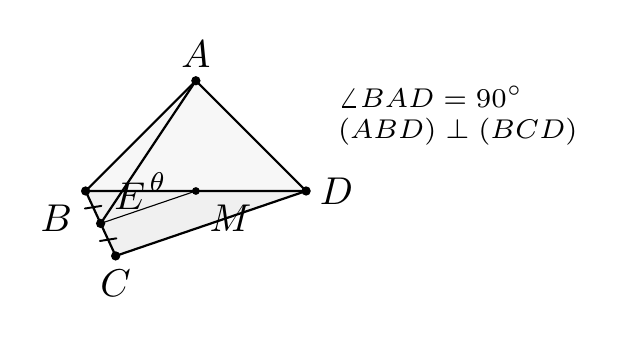
\begin{tikzpicture}[scale=1.4,transform shape,
  x={(1cm,0cm)}, y={(-0.42cm,-0.34cm)}, z={(0cm,1cm)},
  line cap=round, line join=round, >=stealth
]
  \coordinate (B) at (0,0,0);
  \coordinate (D) at (2,0,0);
  \coordinate (C) at (1,1.732,0);
  \coordinate (A) at (1,0,1);
  \coordinate (E) at (0.5,0.866,0);
  \coordinate (M) at (1,0,0);

  % The two triangles lie in perpendicular planes and share BD.
  \fill[black!3] (B)--(D)--(A)--cycle;
  \fill[black!6] (B)--(C)--(D)--cycle;
  \draw[thick] (A)--(B)--(D)--cycle;
  \draw[thick] (B)--(C)--(D);
  \draw[thick] (A)--(E);
  \draw[thin] (M)--(E);

  % E is the midpoint of BC; M is the midpoint of BD and the foot of A.
  \fill (A) circle (1.2pt) node[above] {$A$};
  \fill (B) circle (1.2pt) node[below left] {$B$};
  \fill (C) circle (1.2pt) node[below] {$C$};
  \fill (D) circle (1.2pt) node[right] {$D$};
  \fill (E) circle (1.2pt) node[above right] {$E$};
  \fill (M) circle (1pt) node[below right] {$M$};

  % Short matching ticks on BE and EC indicate the stated midpoint.
  \draw[line width=0.7pt] (0.31,0.398,0) -- (0.19,0.468,0);
  \draw[line width=0.7pt] (0.81,1.264,0) -- (0.69,1.334,0);

  \node[align=left,anchor=west,font=\scriptsize] at (2.25,0.20,0.75)
    {$\angle BAD=90^\circ$\\$(ABD)\perp(BCD)$};
  \node[font=\scriptsize] at (0.70,0.12,0.12) {$\theta$};
\end{tikzpicture}
\end{center}
\nopagebreak[4]
\Needspace{4\baselineskip}
\textbf{解析}

\Needspace{5\baselineskip}
取 $B=(-1,0,0)$、$D=(1,0,0)$，令平面 $BCD$ 为 $xy$ 平面，并取 $C=(0,\sqrt3,0)$。因平面 $ABD\perp BCD$，且 $ABD$ 是以 $A$ 为直角顶点的等腰直角三角形，可取 $A=(0,0,1)$。于是 $E$ 为 $BC$ 中点，

\nopagebreak[4]
\[
\overrightarrow{AE}=\left(-\frac12,\frac{\sqrt3}{2},-1\right),\qquad |AE|=\sqrt2.
\]

向量 $AE$ 在平面 $BCD$ 法向方向上的分量长为 $1$，故线面角 $\theta$ 满足 $\sin\theta=\dfrac1{\sqrt2}$，得 $\theta=45^\circ$。坐标只为由题设关系推导，不表示原图比例。

\gkanswer{答案：$45^\circ$。}

\end{answer}
\begin{answer}
\gksolhead{9}{}

\textbf{题目}：

若两个长方体的长、宽、高分别为 $5\,\mathrm{cm}$、$4\,\mathrm{cm}$、$3\,\mathrm{cm}$，把它们两个全等的面重合在一起组成大长方体，则大长方体的对角线最长为 $\underline{\qquad}\,\mathrm{cm}$。

\Needspace{4\baselineskip}
\textbf{解析}

两个长方体可沿边长为 $4,3$、$5,3$ 或 $5,4$ 的全等面拼合，所得尺寸分别为 $10\times4\times3$、$5\times8\times3$、$5\times4\times6$。对应对角线平方为 $125,98,77$，最大者为 $125$，故最长对角线为 $5\sqrt5\,\mathrm{cm}$。

\gkanswer{答案：$5\sqrt{5}\,\mathrm{cm}$。}

\end{answer}
\begin{answer}
\gksolhead{10}{}

\textbf{题目}：

有 $n$（$n\in\mathbb{N}$）件不同的产品排成一排，若其中 $A$、$B$ 两件产品排在一起的不同排法有 $48$ 种，则 $n=\underline{\qquad}$。

\Needspace{4\baselineskip}
\textbf{解析}

\Needspace{5\baselineskip}
把 $A,B$ 作为一个整体，与其余 $n-2$ 件产品共 $n-1$ 个对象排列，再乘 $A,B$ 内部的 $2$ 种次序，故

\nopagebreak[4]
\[
2(n-1)!=48\quad\Longrightarrow\quad(n-1)!=24,
\]

所以 $n=5$。

\gkanswer{答案：$n=5$。}

\end{answer}
\begin{answer}
\gksolhead{11}{}

\textbf{题目}：

集合 $A=\{(x,y)\mid x^2+y^2=4\}$，$B=\{(x,y)\mid (x-3)^2+(y-4)^2=r^2\}$，其中 $r>0$。若 $A\cap B$ 中有且仅有一个元素，则 $r$ 的值是 $\underline{\qquad}$。

\Needspace{4\baselineskip}
\textbf{解析}

$A$ 是圆心为 $(0,0)$、半径 $2$ 的圆；$B$ 是圆心为 $(3,4)$、半径 $r$ 的圆。圆心距为 $5$。两圆只有一个公共点时，外切给出 $r+2=5$，即 $r=3$；内切给出 $|r-2|=5$，结合 $r>0$ 得 $r=7$。

\gkanswer{答案：$r=3$ 或 $r=7$。}

\end{answer}
\begin{answer}
\gksolhead{12}{}

\textbf{题目}：

设 $I$ 是全集，非空集合 $P$、$Q$ 满足 $P\subset Q\subset I$。若含 $P$、$Q$ 的一个集合运算表达式，使运算结果为空集 $\varnothing$，则这个运算表达式可以是 $\underline{\qquad}$（只要写出一个表达式）。

\Needspace{4\baselineskip}
\textbf{解析}

\Needspace{5\baselineskip}
因 $P\subset Q$，$P$ 与 $Q$ 的补集不相交，因此

\nopagebreak[4]
\[
\overline{Q}\cap P=\varnothing.
\]

这是符合题意的一个表达式。

\gkanswer{答案：例如 $\overline{Q}\cap P$。}

\end{answer}
\gkpart{二、选择题}

\begin{answer}
\gksolhead{13}{}

\textbf{题目}：

抛物线 $y=-x^2$ 的焦点坐标为\mbox{（　　）}。

（A）$(0,\dfrac{1}{4})$.　　（B）$(0,-\dfrac{1}{4})$.　　（C）$(\dfrac{1}{4},0)$.　　（D）$(-\dfrac{1}{4},0)$.

[答]（　）

\Needspace{4\baselineskip}
\textbf{解析}

将 $y=-x^2$ 写成 $x^2=4py$，得 $4p=-1$、$p=-\dfrac14$，焦点为 $(0,-\dfrac14)$，选 B。

\gkanswer{答案：B。}

\end{answer}
\begin{answer}
\gksolhead{14}{}

\textbf{题目}：

$x=\sqrt{1-3y^2}$ 所表示的曲线是\mbox{（　　）}。

（A）双曲线.　　（B）椭圆.　　（C）双曲线的一部分.　　（D）椭圆的一部分.

[答]（　）

\Needspace{4\baselineskip}
\textbf{解析}

\Needspace{5\baselineskip}
平方并保留原式的 $x\ge0$ 条件，得到

\nopagebreak[4]
\[
x^2+3y^2=1,\qquad x\ge0.
\]

这是椭圆的右半部分，选 D。

\gkanswer{答案：D。}

\end{answer}
\begin{answer}
\gksolhead{15}{}

\textbf{题目}：

“$a=1$”是“函数 $y=\cos^2 ax-\sin^2 ax$ 的最小正周期为 $\pi$”的\mbox{（　　）}。

（A）充分不必要条件.　　（B）必要不充分条件.　　（C）充要条件.　　（D）既非充分条件也非必要条件.

[答]（　）

\Needspace{4\baselineskip}
\textbf{解析}

\nopagebreak[4]
\[
y=\cos^2(ax)-\sin^2(ax)=\cos(2ax).
\]

当 $a\ne0$ 时，最小正周期为 $\dfrac\pi{|a|}$；当 $a=0$ 时函数为常数，不存在最小正周期。故最小正周期为 $\pi$ 等价于 $|a|=1$。$a=1$ 足以推出该周期，但不是必要条件（$a=-1$ 也满足），选 A。

\gkanswer{答案：A。}

\end{answer}
\begin{answer}
\gksolhead{16}{}

\textbf{题目}：

若 $0<a<1$，$b<-1$，则函数 $f(x)=a^x+b$ 的图像不经过\mbox{（　　）}。

（A）第一象限.　　（B）第二象限.　　（C）第三象限.　　（D）第四象限.

[答]（　）

\Needspace{4\baselineskip}
\textbf{解析}

若 $x>0$，则 $0<a^x<1$ 且 $b<-1$，所以 $f(x)=a^x+b<0$，图像不可能经过第一象限。另一方面，$x$ 充分小时 $a^x$ 足够大，图像进入第二象限；$x<0$ 充分接近 $0$ 时 $f(x)<0$，进入第三象限；$x>0$ 时 $f(x)<0$，进入第四象限。故选 A。

\gkanswer{答案：A。}

\end{answer}
\gkpart{三、解答题}

\begin{answer}
\gksolhead{17}{}

\textbf{题目}（本题满分 10 分）：

设 $f(x)$ 为定义在 $\mathbb{R}$ 上的偶函数。当 $x\le -1$ 时，$y=f(x)$ 的图像是经过点 $(-2,0)$、斜率为 $1$ 的射线；又在 $y=f(x)$ 的图像中有一部分是顶点在 $(0,2)$，且过点 $(-1,1)$ 的一段抛物线。试写出函数 $f(x)$ 的表达式，并作出其图像。
\nopagebreak[4]
\begin{center}% Q17：按题设得到的分段函数精确绘图，坐标轴及曲线均为矢量。
% 关键点：(-2,0)、(-1,1)、(0,2)、(1,1)、(2,0)。
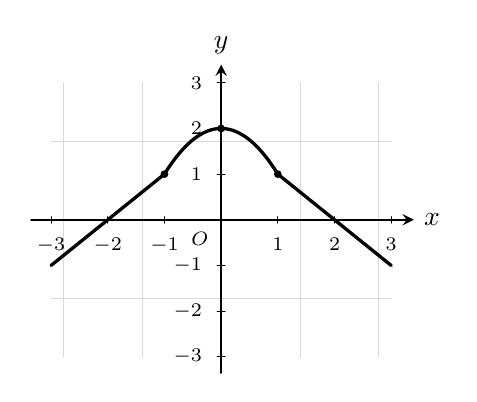
\begin{tikzpicture}[x=0.72cm,y=0.58cm,line cap=round,line join=round,>=stealth]
  % Unit grid matching the original coordinate grid.
  \draw[gray!30,line width=0.25pt] (-3,-3) grid (3,3);
  \draw[->,thick] (-3.35,0)--(3.4,0) node[right] {$x$};
  \draw[->,thick] (0,-3.35)--(0,3.4) node[above] {$y$};

  \foreach \x in {-3,-2,-1,1,2,3}
    \draw (\x,0.07)--(\x,-0.07) node[below=2pt,font=\scriptsize] {$\x$};
  \foreach \y in {-3,-2,-1,1,2,3}
    \draw (0.07,\y)--(-0.07,\y) node[left=2pt,font=\scriptsize] {$\y$};
  \node[below left=1pt,font=\scriptsize] at (0,0) {$O$};

  % f(x)=x+2 for x<=-1, 2-x^2 for -1<x<1, and 2-x for x>=1.
  \draw[very thick] plot[domain=-3:-1,samples=2] (\x,{\x+2});
  \draw[very thick] plot[domain=-1:1,samples=81] (\x,{2-\x*\x});
  \draw[very thick] plot[domain=1:3,samples=2] (\x,{2-\x});
  \foreach \x/\y in {-1/1,0/2,1/1}
    \fill (\x,\y) circle (1.4pt);
\end{tikzpicture}
\end{center}
\nopagebreak[4]
\Needspace{4\baselineskip}
\textbf{解析}

\Needspace{5\baselineskip}
当 $x\le-1$ 时，射线斜率为 $1$ 且过 $(-2,0)$，故 $f(x)=x+2$。在 $-1<x<1$ 的抛物线顶点为 $(0,2)$，设其为 $f(x)=ax^2+2$；代入 $(-1,1)$ 得 $a=-1$。由偶函数性质，$x\ge1$ 时 $f(x)=f(-x)=-x+2$。因此

\nopagebreak[4]
\[
f(x)=\begin{cases}
x+2,&x\le-1,\\
2-x^2,&-1<x<1,\\
-x+2,&x\ge1.
\end{cases}
\]

各段在 $x=\pm1$ 处均取值 $1$，端点归属与题设一致；图见题面 TikZ 图稿。

\gkanswer{答案：$f(x)=\begin{cases}x+2,&x\le-1,\\2-x^2,&-1<x<1,\\-x+2,&x\ge1.\end{cases}$；图见题面图稿。}

\end{answer}
\begin{answer}
\gksolhead{18}{}

\textbf{题目}（本题满分 12 分）：

设复数 $z$ 满足 $|z|=5$，且 $(3+4i)z$ 在复平面上对应的点在第二、四象限的角平分线上，$|\sqrt{2}z-m|=5\sqrt{2}$（$m\in\mathbb{R}$），求 $z$ 和 $m$ 的值。

\Needspace{4\baselineskip}
\textbf{解析}

\Needspace{5\baselineskip}
设 $z=x+yi$。$(3+4i)z$ 的实部、虚部分别为 $3x-4y$、$4x+3y$。第二、四象限角平分线满足虚部为实部的相反数，因此 $4x+3y=-(3x-4y)$，即 $y=7x$。结合 $|z|=5$ 得

\nopagebreak[4]
\[
x^2+y^2=50x^2=25,\qquad x=\pm\frac{\sqrt2}{2},\quad y=\pm\frac{7\sqrt2}{2},
\]

\Needspace{5\baselineskip}
其中 $x,y$ 同号。于是 $\sqrt2z=\pm(1+7i)$。若 $\sqrt2z=1+7i$，则

\nopagebreak[4]
\[
|1+7i-m|^2=(1-m)^2+49=50,
\]

故 $m=0$ 或 $2$。若 $\sqrt2z=-(1+7i)$，则 $(-1-m)^2+49=50$，故 $m=0$ 或 $-2$。答案按上述 $z$ 与 $m$ 的对应关系取值。

\gkanswer{答案：$z=\pm\left(\dfrac{\sqrt2}{2}+\dfrac{7\sqrt2}{2}i\right)$；$z=\dfrac{1+7i}{\sqrt2}$ 时 $m=0,2$，$z=-\dfrac{1+7i}{\sqrt2}$ 时 $m=0,-2$。}

\end{answer}
\begin{answer}
\gksolhead{19}{}

\textbf{题目}（本题满分 12 分）：

有一批影碟机（VCD）原销售价为每台 800 元，在甲乙两家家电商场均有销售。甲商场用如下方法促销：买一台单价为 780 元，买两台每台单价都为 760 元，依次类推，每多买一台则所买各台单价均再减少 20 元，但每台最低价不能低于 440 元；乙商场一律都按原价的 75\% 销售。某单位需购买一批此类影碟机，问去哪个商场购买花费较少？

\Needspace{4\baselineskip}
\textbf{解析}

\Needspace{5\baselineskip}
设购买 $x\in\mathbb N$ 台。甲商场第 $x$ 档的单价为 $800-20x$ 元，但不低于 $440$ 元。因此

\nopagebreak[4]
\[
C_A(x)=\begin{cases}(800-20x)x,&1\le x\le18,\\440x,&x>18,\end{cases}
\qquad C_B(x)=600x.
\]

当 $1\le x\le18$ 时，$C_A-C_B=20x(10-x)$；当 $x>18$ 时，$C_A-C_B=-160x<0$。所以 $x<10$ 时乙较省，$x=10$ 时两店费用相同，$x>10$ 时甲较省。

\gkanswer{答案：购买 $1$–$9$ 台时乙较省；购买 $10$ 台两者相同；购买 $11$ 台及以上时甲较省。}

\end{answer}
\begin{answer}
\gksolhead{20}{}

\textbf{题目}（本题满分 16 分）：

本题共有 2 个小题，每小题满分均为 8 分。已知 $\{a_n\}$ 是等差数列，$a_1=-393$，$a_2+a_3=-768$；$\{b_n\}$ 是公比为 $q$（$0<q<1$）的无穷等比数列，$b_1=2$，且 $\{b_n\}$ 的各项和为 20。

（1） 写出 $\{a_n\}$ 和 $\{b_n\}$ 的通项公式；

\Needspace{5\baselineskip}
（2） 试求满足下列不等式的正整数 $m$：

\nopagebreak[4]
\[
\frac{a_{m+1}+a_{m+2}+\cdots+a_{2m}}{m+1}\le -160b_2.
\]

\Needspace{4\baselineskip}
\textbf{解析}

\gksubpart{(1)}

\Needspace{5\baselineskip}
设等差数列公差为 $d$。则

\nopagebreak[4]
\[
a_2+a_3=2a_1+3d=-786+3d=-768,
\]

\Needspace{5\baselineskip}
得 $d=6$，故 $a_n=-393+6(n-1)=6n-399$。等比数列满足 $\dfrac{2}{1-q}=20$，所以 $q=\dfrac9{10}$，

\nopagebreak[4]
\[
b_n=2\left(\frac9{10}\right)^{n-1},\qquad b_2=\frac95.
\]

\gksubpart{(2)}

\Needspace{5\baselineskip}
又

\nopagebreak[4]
\[
\sum_{k=m+1}^{2m}a_k=6\sum_{k=m+1}^{2m}k-399m=9m^2-396m.
\]

\Needspace{5\baselineskip}
原不等式等价于

\nopagebreak[4]
\[
9m^2-396m\le-160\cdot\frac95(m+1),
\]

即 $m^2-12m+32\le0$，也就是 $(m-4)(m-8)\le0$。满足条件的正整数为 $m=4,5,6,7,8$。

\gkanswer{答案（1）：$a_n=6n-399$，$b_n=2\left(\dfrac9{10}\right)^{n-1}$。}

\gkanswer{答案（2）：$m=4,5,6,7,8$。}

\end{answer}
\begin{answer}
\gksolhead{21}{}

\textbf{题目}（本题满分 18 分）：

本题共有 3 个小题，第 1 小题满分 4 分，第 2 小题满分 6 分，第 3 小题满分 8 分。四棱锥 $P-ABCD$ 中，底面 $ABCD$ 是一个平行四边形，$\overrightarrow{AB}=(2,-1,-4)$，$\overrightarrow{AD}=(4,2,0)$，$\overrightarrow{AP}=(-1,2,-1)$。

（1） 求证：$PA\perp$ 底面 $ABCD$；

（2） 求四棱锥 $P-ABCD$ 的体积；

\Needspace{5\baselineskip}
（3） 对于向量 $\mathbf{a}=(x_1,y_1,z_1)$，$\mathbf{b}=(x_2,y_2,z_2)$，$\mathbf{c}=(x_3,y_3,z_3)$，定义一种运算：

\nopagebreak[4]
\[
(\mathbf{a}\times\mathbf{b})\cdot\mathbf{c}=x_1y_2z_3+x_2y_3z_1+x_3y_1z_2-x_1y_3z_2-x_2y_1z_3-x_3y_2z_1.
\]

试计算 $\left|(\overrightarrow{AB}\times\overrightarrow{AD})\cdot\overrightarrow{AP}\right|$ 的值；说明其与四棱锥 $P-ABCD$ 体积的关系，并由此猜想向量这一运算的绝对值的几何意义。

\Needspace{4\baselineskip}
\textbf{解析}

\gksubpart{(1)}

\nopagebreak[4]
\[
\overrightarrow{AP}\cdot\overrightarrow{AB}=-2-2+4=0,\qquad
\overrightarrow{AP}\cdot\overrightarrow{AD}=-4+4=0.
\]

由于 $AB,AD$ 是底面内两条相交直线，故 $AP\perp$ 平面 $ABCD$。

\gksubpart{(2)}

\Needspace{5\baselineskip}
$|AP|=\sqrt6$，且

\nopagebreak[4]
\[
\overrightarrow{AB}\times\overrightarrow{AD}=(8,-16,8),\qquad
|\overrightarrow{AB}\times\overrightarrow{AD}|=8\sqrt6.
\]

\Needspace{5\baselineskip}
底面积为 $8\sqrt6$，高为 $\sqrt6$，所以

\nopagebreak[4]
\[
V=\frac13\cdot8\sqrt6\cdot\sqrt6=16.
\]

\gksubpart{(3)}

按题目给出的运算式代入，$(\overrightarrow{AB}\times\overrightarrow{AD})\cdot\overrightarrow{AP}=(8,-16,8)\cdot(-1,2,-1)=-48$。绝对值为 $48=3V$。一般而言，三个向量的标量三重积绝对值表示以它们为棱的平行六面体体积；其对应四棱锥体积为该值的三分之一。

\gkanswer{答案（1）：$PA\perp$ 底面 $ABCD$，证明见解析。}

\gkanswer{答案（2）：四棱锥体积为 $16$。}

\gkanswer{答案（3）：混合积绝对值为 $48$，是四棱锥体积的 $3$ 倍；该混合积绝对值表示以三个向量为棱的平行六面体体积。}

\end{answer}
\begin{answer}
\gksolhead{22}{}

\textbf{题目}（本题满分 18 分）：

\Needspace{5\baselineskip}
本题共有 3 个小题，每小题满分均为 6 分。如图所示，$A,F$ 分别是椭圆

\nopagebreak[4]
\[
\frac{(y+1)^2}{16}+\frac{(x-1)^2}{12}=1
\]

的一个顶点与一个焦点。位于 $x$ 轴的正半轴上的动点 $T(t,0)$ 与 $F$ 的连线交射线 $OA$ 于 $Q$。求：
\nopagebreak[4]
\begin{center}% Q22 椭圆与点线关系矢量示意。椭圆按方程取轴长；T 仅作 t>2/3 的代表位置，图不按比例。
% Source equation: \frac{(y+1)^2}{16}+\frac{(x-1)^2}{12}=1.
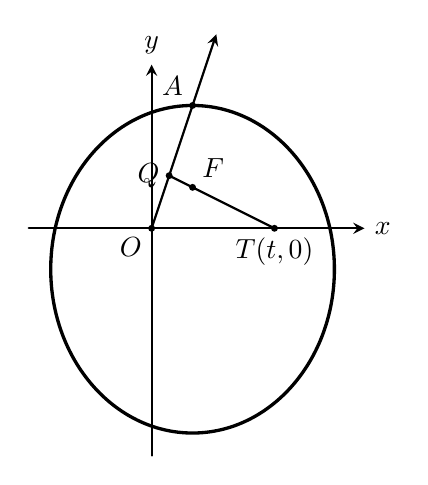
\begin{tikzpicture}[x=0.52cm,y=0.52cm,line cap=round,line join=round,>=stealth]
  \draw[->,thick] (-3.0,0)--(5.2,0) node[right] {$x$};
  \draw[->,thick] (0,-5.55)--(0,4.0) node[above] {$y$};

  % Ellipse center (1,-1), semiaxes 2sqrt(3) and 4.
  \draw[very thick] (1,-1) ellipse [x radius=3.4641,y radius=4];

  % A=(1,3) is the upper vertex and F=(1,1) the upper focus, as in the source figure.
  \coordinate (O) at (0,0);
  \coordinate (A) at (1,3);
  \coordinate (F) at (1,1);
  % A representative t=3 gives Q=(3/7,9/7); T is labeled parametrically.
  \coordinate (T) at (3,0);
  \coordinate (Q) at (0.4286,1.2857);

  \draw[thick,->] (O)--(1.58,4.74);
  \draw[thick] (T)--(Q);

  \fill (O) circle (1.25pt) node[below left] {$O$};
  \fill (A) circle (1.25pt) node[above left] {$A$};
  \fill (F) circle (1.25pt) node[above right] {$F$};
  \fill (T) circle (1.25pt) node[below] {$T(t,0)$};
  \fill (Q) circle (1.25pt) node[left] {$Q$};
\end{tikzpicture}
\end{center}
\nopagebreak[4]
（1） 点 $A,F$ 的坐标及直线 $TQ$ 的方程；

（2） $\triangle OTQ$ 的面积 $S$ 与 $t$ 的函数关系式 $S=f(t)$ 及该函数的最小值；

（3） 写出 $S=f(t)$ 的单调递增区间，并证明之。

\Needspace{4\baselineskip}
\textbf{解析}

\gksubpart{(1)}

\Needspace{5\baselineskip}
椭圆中心为 $(1,-1)$，纵向半轴长为 $4$，横向半轴长为 $2\sqrt3$，故 $c=\sqrt{16-12}=2$。由图中 $A,F$ 的位置可取 $A=(1,3)$、$F=(1,1)$。当 $t\ne1$ 时，直线 $TF$ 为

\nopagebreak[4]
\[
y=\frac{x-t}{1-t};
\]

当 $t=1$ 时为 $x=1$。

\gksubpart{(2)}

\Needspace{5\baselineskip}
射线 $OA$ 的方程为 $y=3x$。两者交于

\nopagebreak[4]
\[
Q=\left(\frac{t}{3t-2},\frac{3t}{3t-2}\right).
\]

\Needspace{5\baselineskip}
因 $T$ 在 $x$ 轴正半轴且 $Q$ 在射线 $OA$ 上，需 $t>0$ 且 $\dfrac{t}{3t-2}>0$，因此 $t>\dfrac23$。三角形面积为

\nopagebreak[4]
\[
S=f(t)=\frac12\,t\,\frac{3t}{3t-2}=\frac{3t^2}{2(3t-2)},\qquad t>\frac23.
\]

\gksubpart{(3)}

求导得 $f'(t)=\dfrac{3t(3t-4)}{2(3t-2)^2}$。故 $f$ 在 $(\frac23,\frac43)$ 上递减，在 $(\frac43,+\infty)$ 上递增；最小值在 $t=\frac43$ 处取得，为 $f(\frac43)=\frac43$。图见题面 TikZ 图稿。

\gkanswer{答案（1）：$A=(1,3)$，$F=(1,1)$；当 $t\ne1$ 时直线 $TQ$ 为 $y=\dfrac{x-t}{1-t}$，当 $t=1$ 时为 $x=1$。}

\gkanswer{答案（2）：$t>\dfrac23$，$S=\dfrac{3t^2}{2(3t-2)}$，最小值为 $\dfrac43$。}

\gkanswer{答案（3）：单调递增区间为 $\left(\dfrac43,+\infty\right)$。}

\end{answer}